% section on numerics

\newcommand{\tom}{\tilde\om}
\newcommand{\tOm}{\tilde\Om}

%%%%%%%%%%%%%%%%%%%%%%%%%%%%%%%%%%%%%%%%%%%%%%%%%%%%%%%%%
\section{Algorithms}
\label{sec:implementation}

This section discusses some of the finer points of the implementation. Basic discretization issues were exposed in Section \ref{sec:disc}.

%\subsection{Basic}

%%%%%%%%%%%%%%%%%%%%%%%%%%%%%%%%%%%%%%%%%%%%%%%%%%%%%%%%%

%Briefly describe the bases we will use: Diracs, wavelets, bandlets, curvelets.

%%%%%%%%%%%%%%%%%%%%%%%%%%%%%%%%%%%%%%%%%%%%%%%%%%%%%%%%%
\subsection{Extraction of the Eigenvectors}
\label{subsec-extraction-eigen}

The first part of the algorithm consists in extracting a random set of eigenvectors $\{ \tilde v_{\tom} \}_{\tom}$ of the discretized operator $\Ll = \Si^{-2} L$ where $\Si = \diag_j( \sigmaj )$.  The discretized Laplacian $L$ over $\RR$ is computed spectrally 
\eq{
	\widehat{L v}[m] = - 4 \pi^2 m^2 \hat v[m] 
}
where $m \in \{ -N/2+1,\ldots,N/2 \}$ indexes the frequencies of the discrete Fourier transform. Fourier transforms are computed in $O(N \log N)$ operation with the FFT.

%LD: It's Sigma^{-2} no? Before you had written SIgma^{-1}
%GP: Yep you are right

%LD: ALso I think you had forgotten a minus sign -- confirm that this is indeed your def of the Laplacian
%GP: Yep.

Since we are interested in extracting only a few eigenvectors chosen at random, we use an iterative method \cite{templates-eigen} that parallelizes trivially on multiple processors. Each processor computes and stores independently from the others a few eigenvectors using an iterative method. 

%LD: manque une ref ci-dessus
%GP: je ne connais pas trop la biblio ...
% OK I remove

The simplest way to compute an eigenvector $\tilde v_{\tom}$ whose eigenvalue $-\tom^2$ is closest to a given $-\tom_0^2$ is to compute iterative inverse powers
\eq{
	\tilde v_{\tom}^{(k+1)} = (\Ll + \tom_0^2 \Id)^{-1} \tilde v_{\tom}^{(k)},
}
with an adequate starting guess $\tilde v_{\tom}^{(0)}$, typically white noise. In practice we use a variant of this power iteration called the restarted Arnoldi method, and coded in Matlab's \texttt{eigs} command.
At each iteration we approximately solve the linear system $(\Ll + \tom_0^2 \Id) \tilde v_{\tom}^{(k+1)} = \tilde v_{\tom}^{(k)}$ with a few steps of stabilized bi-conjugate gradient \cite{templates-linsyst}. Recent work \cite{ErlNab} suggests that a shift in the reverse direction $\Ll - \tom_0^2 \Id$ or a complex shift $\Ll + \imath\tom_0^2 \Id$ are good preconditionners for this linear system resolution. Such preconditoners are applied efficiently using multigrid, or alternatively and as used in this paper, using discrete symbol calculus. In this framework, it is the whole symbol of the operator $(\Ll - \tom_0^2 \Id)^{-1}$ which is precomputed in compressed form, and then applied iteratively to functions on demand. The resulting preconditioners are quite competitive. See \cite{DSC} for more information.

%LD: manque une autre ref ci-dessus
%GP: a quelle ref penses tu ?
%probleme resolu apparemment

Each shift $\tom_0^2$ should be chosen according to an estimate of the true (but unknown) eigenvalues repartition to sample as uniformly as possible the set of eigenvectors of $\Ll$. The eigenvalues of the discrete Laplacian in a constant medium $\sigmaj = \si_0$ are $\{ - \om_{\max}^2 (2 m/N)^2 \}_{m=-N/2+1}^{N/2}$ where $\om_{\max}^2 = \pi^2 N^2 / \si_0^2$. Treating the general case as a perturbation of this constant setting leads draw $\tom_0$ uniformly at random in $[0,\om_{\max}]$ where $\om_{\max}$ defined as the maximum eigenvalue of $\Ll$. The value of $\om_{\max}$ is readily available and computed using power iterations on $\Ll$. We have seen in Section \ref{sec:egv-gaps} that the departure from uniformity is under control when the medium has a reasonable total variation. We also explained that the sampling should be without replacement: in practice the implementation of ``replacement" carefully accounts for the multiplicity two of each eigenspace in the case of periodic boundary conditions.



%%%%%%%%%%%%%%%%%%%%%%%%%%%%%%%%%%%%%%%%%%%%%%%%%%%%%%%%%
\subsection{Iterative Thresholding for $\lun$ Minimization}

At the core of the compressive wave computation algorithm is the resolution of the optimization problem \eqref{eq:ell1} involving the $\lun$ norm. We introduce the operator $\Phi : \RR^{N} \mapsto \RR^{\Om}$ such that 
\eq{
	\Phi u[\tom] = \sum_j u[j] \tilde v_{\tom}[j]
}
where $\tom \in \Om$ indexes $K = |\Om|$ eigenvectors $\{ \tilde v_{\tom} \}_{\tom}$ of the discretized Laplacian and $\Si = \diag_j(\sigmaj)$. 
Discarding the time dependency, the $\lun$ optimization \eqref{eq:ell1} is re-written in Lagrangian form as
\begin{equation}\label{eq-lagrangian-optim}
	\underset{u}{\min} \;
	\frac{1}{2} \norm{ \Phi \Si^2 u - \tilde c }^2
	+ \la \sum_j \sigmaj |u[j]|.
\end{equation}
The Lagrangian parameter $\la$ should be set so that $\norm{ \Phi \Si^2 u - \tilde c } \leq \epsilon$.

%LD: I put \leq epsilon instead of = epsilon
%GP: Ok.

As described in Section \ref{sec:disc}, $\epsilon$ account for the discretization error, and it can also reflects errors in computation of the eigenvectors. This quantity can be difficult to estimate precisely, and it can be slightly over-estimated, which increases the sparsity of the computed approximation. 

%LD: Gabriel, a word on how you choose epsilon in practice? (one sentence?)
%GP: hum, je sais pas trop quoi dire. Dans mes xp num�rique, comme y'a tr�s peu de bruit (je calcule un erreur par rapport � une solution deja discr�tis�, et il y a peu d'erreur dans le calcul des vecteurs propres) je prend un epsilon tout petit (eventuellement on peut le decroitre pendant les iterations pour encore le diminuer).  

Iterative algorithms solves the minimization \eqref{eq-lagrangian-optim} by sequentially applying a gradient descent step to minimize $\norm{ \Phi \Si^2 u - \tilde c }$ and a soft thresholding to impose that the solution has a low weighted $\lun$ norm $\sum_j \sigmaj |u[j]|$. This algorithm was proposed independently by several researcher, see for instance \cite{daubechies-iterated,combettes-proximal,figueiredo-nowak-em}, and its convergence is proved in  \cite{daubechies-iterated,combettes-proximal}. 

The steps of the algorithm are detailed in Table \ref{listing-it-thresh}. They correspond to the application of the iterative thresholding algorithm to compute the iterates $\Si u^{(k)}$ with the measurement matrix $\Phi \Si$. Since this matrix satisfies $\norm{\Phi\Si u} \leq \norm{u}$ by Plancherel, these iterates converge to a minimizer of \eqref{eq-lagrangian-optim}.

Since the correspondence between $\epsilon$ and $\la$ is a priori unknown, $\la$ is modified iteratively at step 4 of the algorithm so that the residual error converges to $\epsilon$, as detailed in \cite{chambolle-algo-tv}.

%GP: I added a reference to Chambolle, where \lambda is updated iteratively so that the Lagrangian minimization converges to the solution of the L1 optimization under the constraint |residual|<=\epsilon, which corresponds to the minimization used in CS and in this paper.

An important feature of the iterative algorithm detailed in Table \ref{listing-it-thresh} is that it parallelizes nicely on clusters where the set of eigenvectors $\{ v_{\tom} \}_{\tom \in \tOm}$ are distributed among several nodes. In this case, the transposed operator $\Phi^*$ is pre-computed on the set of nodes, and the application of $\Phi\Si^2$ and $\Si^2 \Phi^*$ is done in parallel during the iterations.

%LD: would you like to write a sentence on why you chose this particular iterative thresh? the other methods wouldn't be as adequate? Else, comment that you leave these aspects to a future contribution? Thanks.
%GP: j'ai ajout� les ref ci dessous.

The iterative thresholding algorithm presented in Table \ref{listing-it-thresh} might not be the fastest way to solve \eqref{eq-lagrangian-optim}. Recent contributions to sparse optimization include for instance primal-dual schemes \cite{zhu-primal-dual}, gradient pursuit \cite{blumensath-grad-pursuit}, gradient projection \cite{figueiredo-grad-projection}, fixed point continuation \cite{hale-fixed-point-cont}, gradient methods \cite{nesterov-smooth}, Bregman iterations \cite{yin-bregman} and greedy pursuits \cite{needell-cosamp}. These methods could potentially improve the speed of our algorithm, although it is still unclear which method should be preferred in practice. 

%LD: excellent merci pour ces refs.

Another avenue for improvement is the replacement of the $\lun$ norm by non-convex functionals that favor more strongly the sparsity of the solution. Non-convex optimization methods such as FOCUSS \cite{gorodnitsky-focuss}, re-weighted $\lun$ \cite{candes-reweighted-l1} or morphological component analysis with hard thresholding \cite{starck-mca} can lead to a sub-optimal local minimum, but seem to improve over $\lun$ minimization in some practical situations.


\begin{listing}
\begin{enumerate}
	\item \textit{Initialization:} set $u^{(0)} = 0$ and $k=0$. %, $t^{(0)} = t_{\max} = \max( \transp{\Psi} \transp{\Phi} f )$, $k=0$.
	\item \textit{Update of the solution:} compute a step of descent of $\norm{ \Phi \Si^2 u - \tilde c }^2$
		\eq{
			\bar u^{(k)} = u^{(k)} + \Phi^* \pa{ \tilde c - \Phi \Si^2 u^{(k)} },
		}
	\item \textit{Minimize $\lun$ norm:} threshold the current update
		\eq{
			\foralls j, \quad u^{(k+1)}[j] = S_{\la / \sigmaj}( \bar u^{(k)}[j] ),
		}
		where the soft thresholding operator is defined as
		\eq{
			S_{\la}(\al) = \choice{
				0 \qifq |\al|<\la,\\
				\al - \sign(\al)\la \quad \text{otherwise}.
			}
		}
	\item \textit{Update the Lagrange multiplier:} set 
	\eq{
		\la \leftarrow \la \frac{\epsilon}{\norm{ \Phi \Si^2 u - \tilde c }}
	}
	\item \textit{Stop:} while $\norm{u^{(k+1)}-u^{(k)}} >$ tol, set $k \leftarrow k+1$ and go back to 2.
\end{enumerate}\vspace{-3mm}
    \caption{Iterative thresholding algorithm to solve \eqref{eq-lagrangian-optim}. \label{listing-it-thresh}}
\end{listing}


\subsection{Sparsity Enhancement}\label{sec:sparsity-enhancement}

The success of the compressive method for wave propagation is directly linked to the sparsity of the initial conditions $u_0$ and $u_1$. To enhance the performance for a fixed set of eigenvectors, the initial data can be decomposed as $u_0 = \sum_{\ell=0}^{\ell-1} u_0^{k}$ where each of the $L$ components $\{u_0^\ell\}_\ell$ is sufficiently sparse, and similarly for $u_1$. The algorithm is then performed $L$ times with each initial condition $u_0^\ell$ and the solution is then recomposed by linearity. It would be interesting to quantify the slight loss in the probability of success since $L$ simulations are now required to be performed accurately, using the same set of eigenvectors.

Since the solution might become less sparse with time $t$ increasing, one can also split the time domain into intervals $[0,t] = \bigcup_i [t_i,t_{i+1}]$, over each of which the loss of sparsity is under control. The algorithm is restarted over each interval $[t_i,t_{i+1}]$ using a decomposition of the wavefields at time $t_i$ into a well chosen number $L = L_{t_i}$ of components to generate sparse new initial conditions. 

%%%%%%%%%%%%%%%%%%%%%%%%%%%%%%%%%%%%%%%%%%%%%%%%%%%%%%%%%
%%%%%%%%%%%%%%%%%%%%%%%%%%%%%%%%%%%%%%%%%%%%%%%%%%%%%%%%%
%%%%%%%%%%%%%%%%%%%%%%%%%%%%%%%%%%%%%%%%%%%%%%%%%%%%%%%%%
\section{Numerical Experiments}

\newcommand{\Err}{\text{\upshape Err}}


%%%%%%%%%%%%%%%%%%%%%%%%%%%%%%%%%%%%%%%%%%%%%%%%%%%%%%%%%
%%%%%%%%%%%%%%%%%%%%%%%%%%%%%%%%%%%%%%%%%%%%%%%%%%%%%%%%%
\subsection{Compressive Propagation Experiments}

We perform simulations on a 1D grid of $N=2048$ points, with impedance $\si(x)$ of various smoothness and contrast $\si_{\max} / \si_{\min}$. The result of the compressive wave computation is an approximate discrete solution $\{\tilde u[j](t) \}_{j=0}^{N-1}$ at a fixed time step $t$ of the exact solution $\{u[j](t)\}_j$ of the discretized wave equation.

The performance of the algorithm is evaluated using the $\ldeux$ recovery error in space and at several time steps $t_i = T i/n_t$ for $i=0,\ldots,n_t-1$ uniformly distributed in  $[0,T]$, where $n_t=100$. The final time is evaluated such that $\int_0^T \si = 1$, so that the initial spike at $t=0$ propagates over the whole domain. This error is averaged among a large number of random sets $\Om \in \Om_K$ of $K$ eigenvectors
\eql{\label{eq-error-measure}
	\Err(\si,K/N)^2 = \frac{1}{N n_t  |\Om_K| \, \norm{u}} \sum_{\Om \in \Om_K} \sum_{i=0}^{n_t-1} \sum_{j=0}^{N-1} | u[j](t_i) - \tilde u[j](t_i) |^2.
}
Each set $\Om \in \Om_K$ is drawn at random using the procedure described in Section \ref{subsec-extraction-eigen}.

This error depends on the sub-sampling factor $K/N$, where $K=|\Om|$ is the number of computed eigenvectors, and on the impedance $\si$ of the medium. Numerical evaluation of the decay of $\Err$ with $K$ are performed for two toy models of acoustic media that could be relevant in seismic settings: smooth $\si$ with an increasing number of oscillations, and piecewise smooth $\si$ with an increasing number of discontinuities. For each test, the initial condition $u_0$ is a narrow gaussian bump of standard deviation $7/N$. 

%%%%%%%%%%%%%%%%%%%%%%%%%%%%%%%%%%%%%%%%%%%%%%%%%%%%%%%%%
\paragraph{Smooth oscillating medium.}

A uniformly smooth impedance $\si_\ga$ parameterized by the number of oscillations $\ga \in [1,20]$ is defined as
\eql{\label{eq-smooth-medium}
	\sigma_\ga[j] = \frac{\si_{\max}+1}{2} + \frac{\si_{\max}-1}{2} \pa{ \sin(2\pi \ga j/N) + 3 }.
}
The contrast $\si_{\max}/\si_{\min}=\si_{\max} \in [1,10]$ is also increased linearly with the complexity $\ga$ of the medium, according to $1+\frac{9}{19}(\gamma-1)$.

%	\ga = \ga(\eta) = 1 + \eta (\ga_0-1) \in [1, \ga_0] \qandq
%	\si_{\max} = \si_{\max}(\eta) = 2 + \eta(\si_0-2) \in [2,\si_0].

%LD: I think we talked about this already, but would you mind grouping eta and gamma? What do you think that we only use gamma, the number of oscillations, and detail how the contrast is changed with gamma. You don't have to restart the simulations, just change eta into gamma. Also, note that eta was used earlier and this could be confusing. 
%GP: Is it ok the way I did the modification ?

Figure \ref{fig-sin-all-error} shows how the recovery error $\Err(\si_{\ga},K/N)$ scales with complexity $\ga$ of the medium and the number of eigenvectors $K$. For media with moderate complexity, one can compute an accurate solution with $N/10$ to $N/5$ eigenvectors.

\myfigure{
	\begin{tabular}{ccc}
		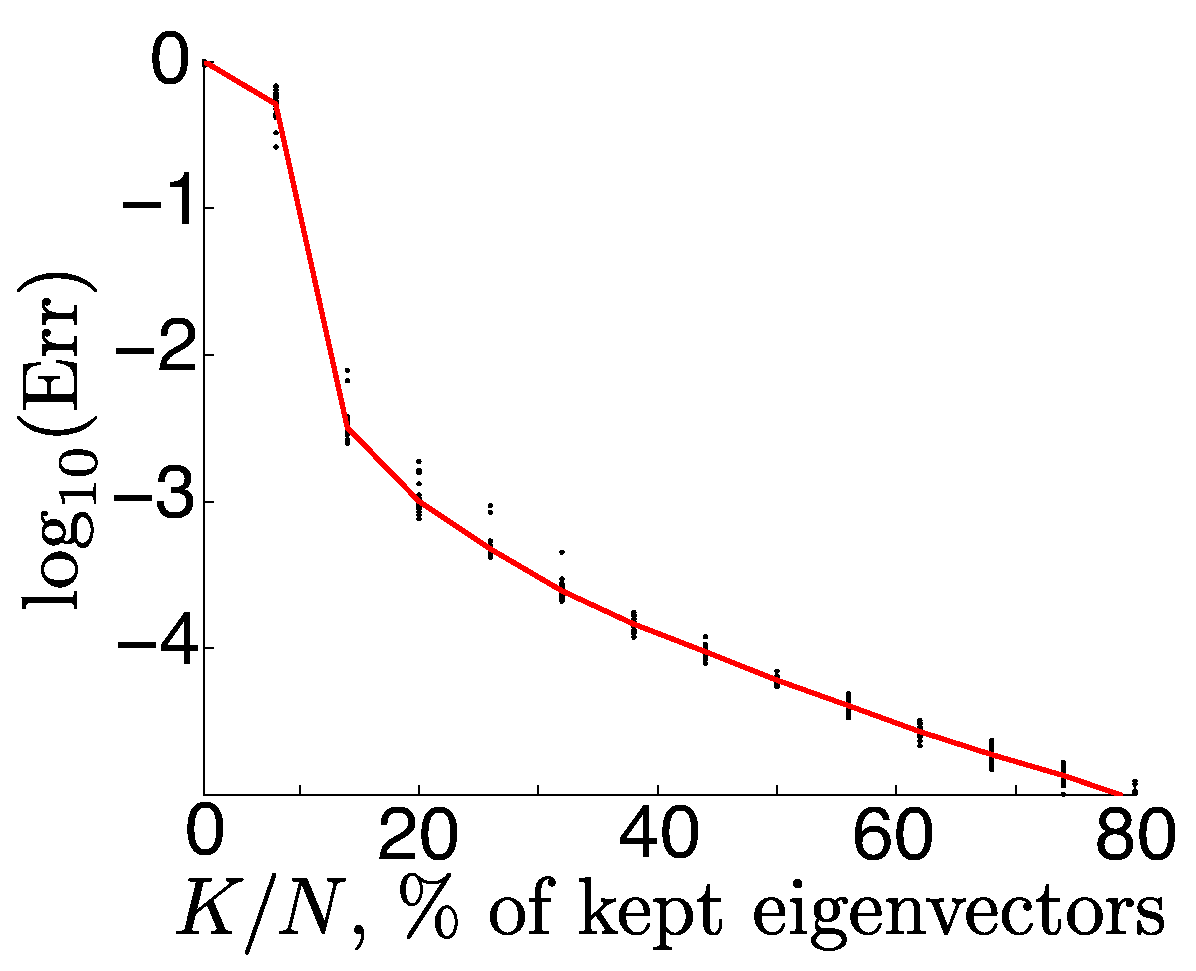
\includegraphics[width=.33\linewidth]{sin-error/sin-cpxity10-error-log.eps}&\hspace{-6mm}
		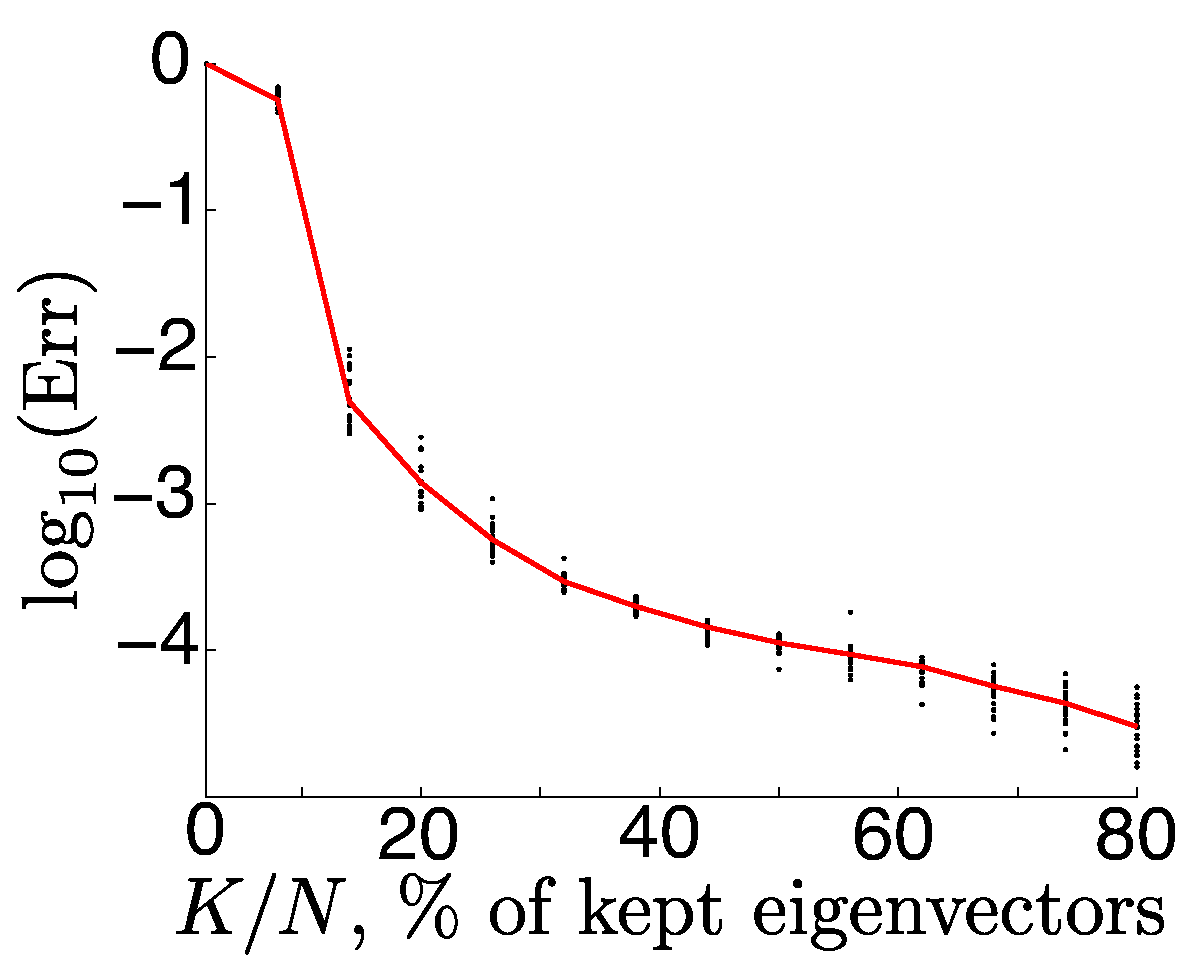
\includegraphics[width=.33\linewidth]{sin-error/sin-cpxity20-error-log.eps}&\hspace{-6mm}
		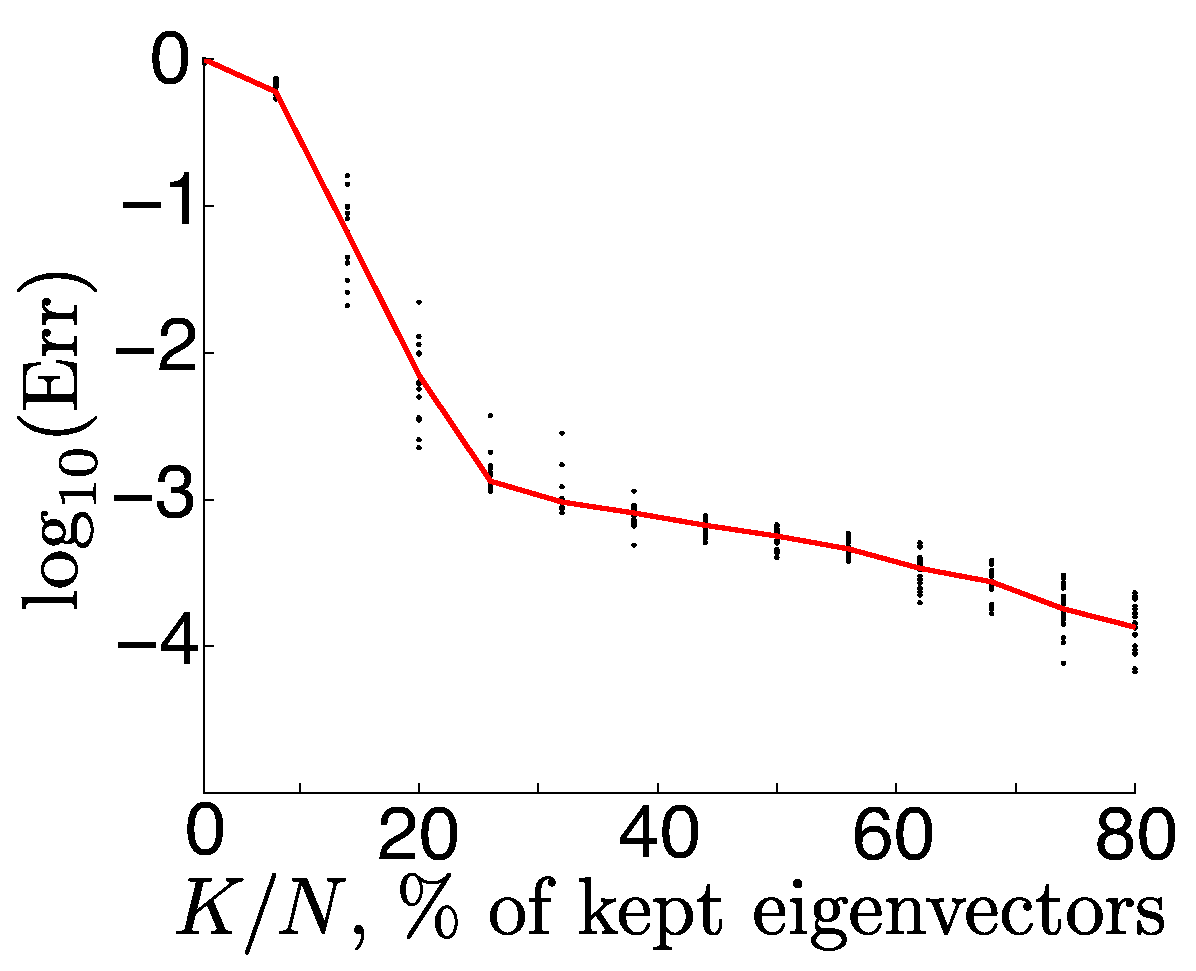
\includegraphics[width=.33\linewidth]{sin-error/sin-cpxity40-error-log.eps}\\
		$\ga=2$ & $\ga=4$ & $\ga=8$	
	\end{tabular}
	\begin{tabular}{c}
    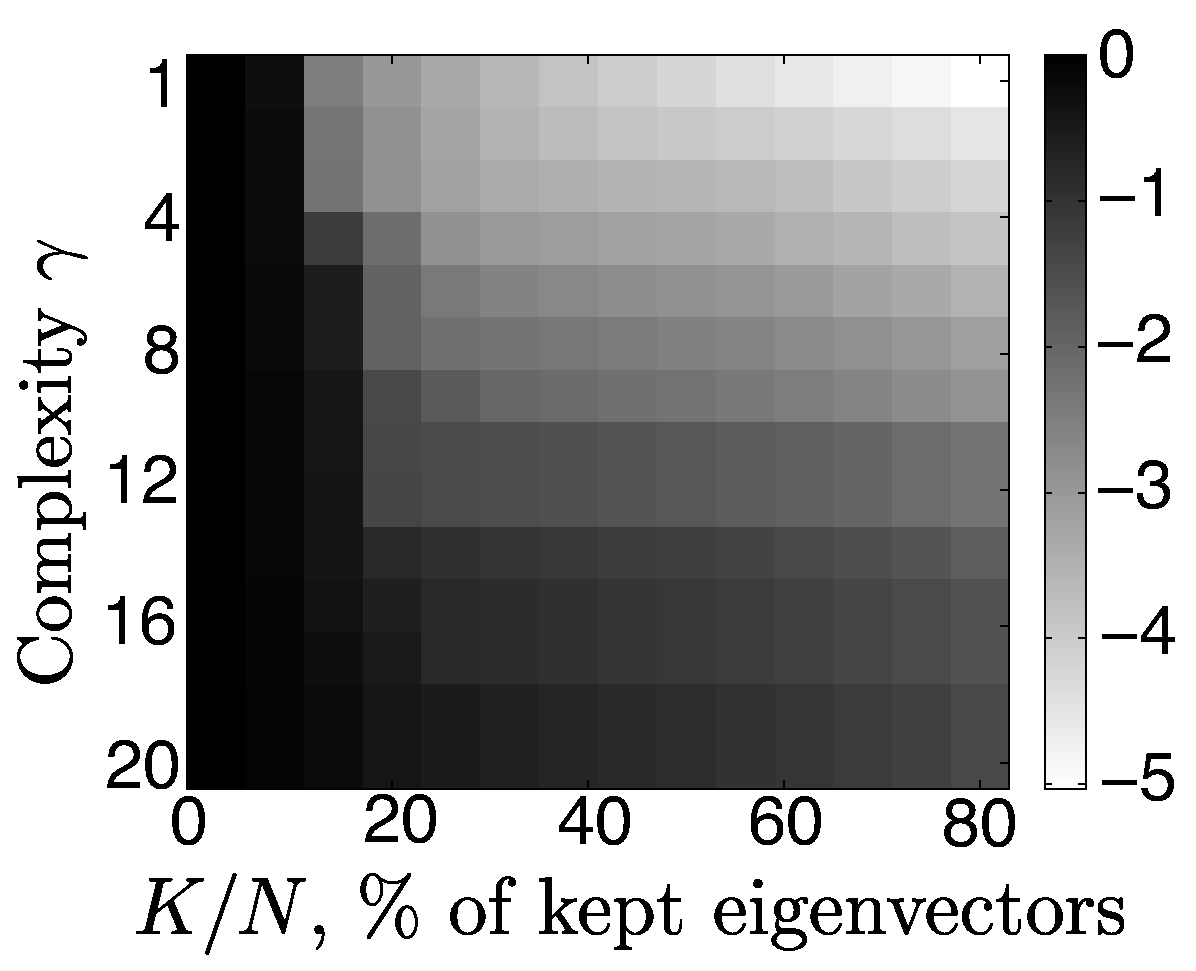
\includegraphics[width=.4\linewidth]{sin-error/sin-all-error.eps}\\
    $\log_{10}(\Err(\si_{\ga},K/N))$
    \end{tabular}
}{ 
	Compressive wave propagation in a smooth medium. Top row: recovery error decay $\log_{10}(\Err(\si_{\ga},K/N))$ as a function of the sub-sampling $K/N$ for various complexity $\ga$ of the medium. Each black dots corresponds to the error of a given random set $\Om$ (the red curve is the result of the averaging among these sets). Bottom row: 2D display of the error $\log_{10}(\Err(\si_{\ga},K/N))$ as a function of both $K/N$ (horizontal axis) and $\ga $ (vertical axis).
}{fig-sin-all-error}


%%%%%%%%%%%%%%%%%%%%%%%%%%%%%%%%%%%%%%%%%%%%%%%%%%%%%%%%%
\paragraph{Piecewise smooth medium.}

Jump discontinuities in the impedance $\si$ reflect the propagating spikes and thus deteriorate the sparsity of the solution when $t$ increases, as shown on Figure \ref{bv-steps}, top row. Figure \ref{bv-steps} shows that compressive wave computation is able to recover the position of the spikes with roughly $N/5$ to $N/4$ eigenvectors. 

\newcommand{\bvspeed}[1]{ \includegraphics[width=.3\linewidth]{bv-steps/bv-steps-rough4-contrast30-#1} }
\newcommand{\myrot}[1]{\rotatebox{90}{\quad\;#1}}
\newcommand{\prespace}{\hspace{-7mm}}
\newcommand{\interspace}{\hspace{-5mm}}
\myfigure{
	\begin{tabular}{cc}
	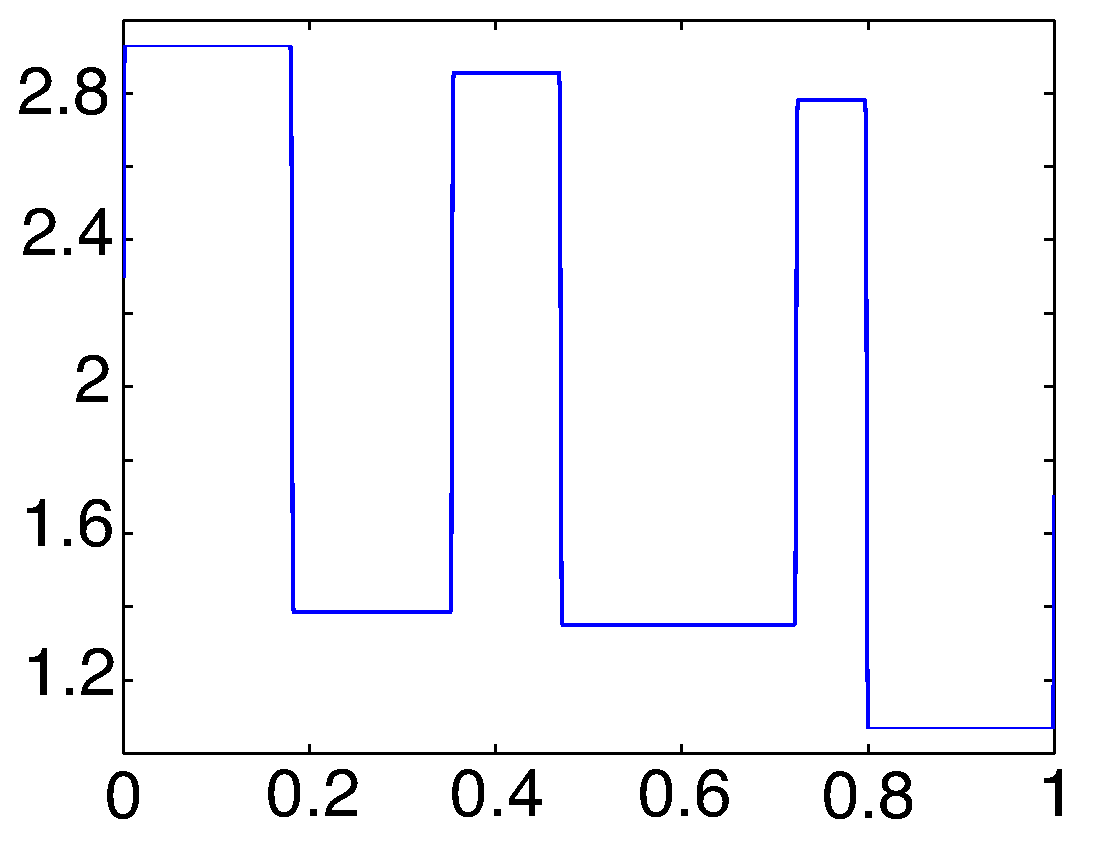
\includegraphics[width=.33\linewidth]{bv-steps/bv-steps-speed.eps}& 
	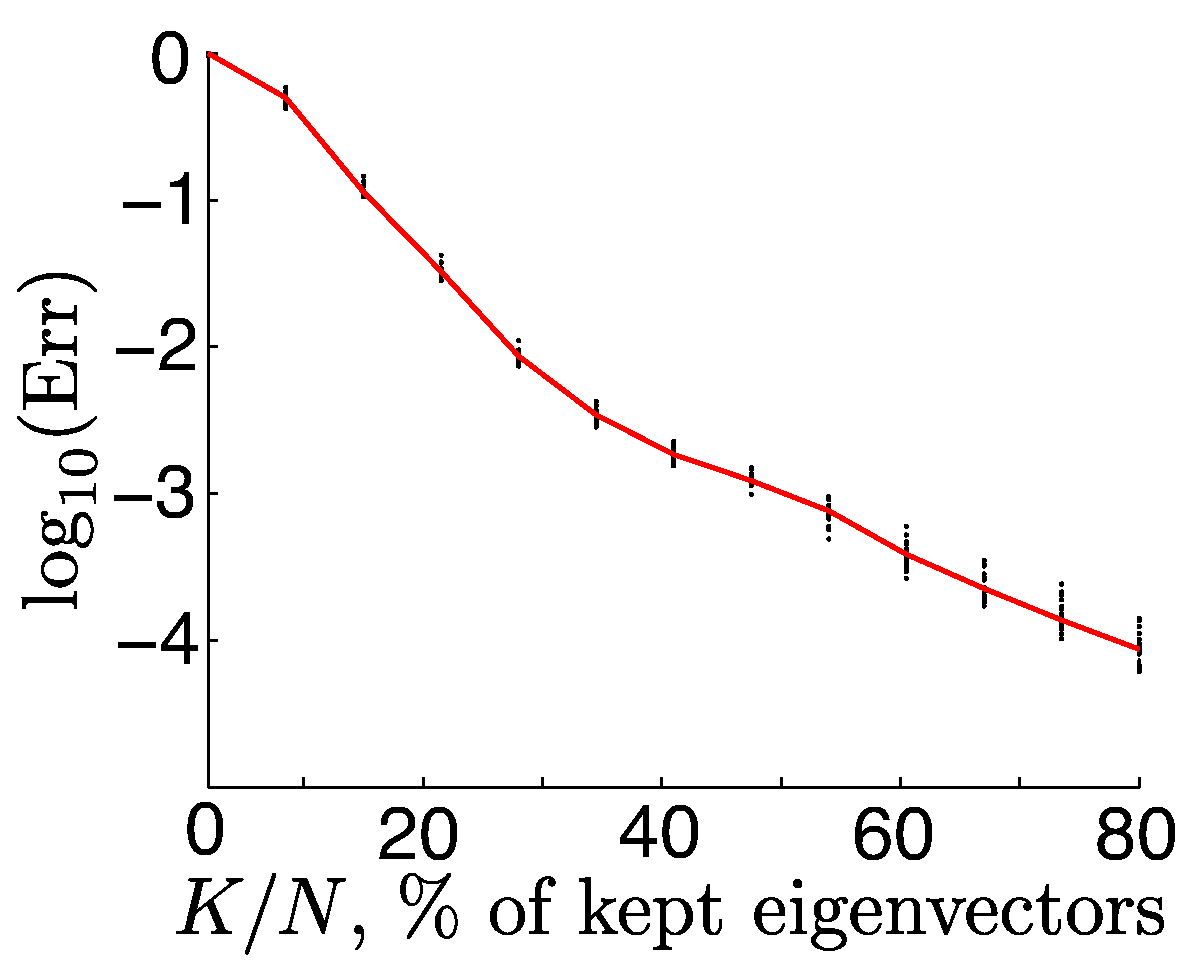
\includegraphics[width=.38\linewidth]{bv-steps/bv-steps-error-log.eps}\\
	Speed $\si^{-1}$ & $\log_{10}(\Err(\si_{\ga},K/N))$
	\end{tabular}
	\begin{tabular}{cccc}
		\myrot{\qquad $u$}& \prespace{}
		\bvspeed{true-2.eps}& \interspace{}
		\bvspeed{true-3.eps}& \interspace{}
		\bvspeed{true-4.eps}\\ %& \interspace{}
%		\bvspeed{true-5.eps}\\
		\myrot{$K/N=0.2$}& \prespace{}
		\bvspeed{sub20-2.eps}& \interspace{}
		\bvspeed{sub20-3.eps}& \interspace{}
		\bvspeed{sub20-4.eps}\\ % & \interspace{}
%		\bvspeed{sub20-5.eps}\\
		\myrot{$K/N=0.15$}& \prespace{}
		\bvspeed{sub15-2.eps}& \interspace{}
		\bvspeed{sub15-3.eps}& \interspace{}
		\bvspeed{sub15-4.eps}\\ % & \interspace{}
%		\bvspeed{sub15-5.eps}\\
%		\myrot{$K/N=0.08$}& \prespace{}
%		\bvspeed{sub08-2.eps}& \interspace{}
%		\bvspeed{sub08-3.eps}& \interspace{}
%		\bvspeed{sub08-4.eps}& \interspace{}
%		\bvspeed{sub08-5.eps}\\
		& $t=.2$ & $t=.4$ & $t=.6$ % & $t=.8$
	\end{tabular}
}{ 
	Examples of approximate solution $\tilde u[j](t)$ for a piecewise smooth medium.
}{bv-steps}

To quantify more precisely the recovery performance, we consider a family of piecewise smooth media $\si_\ga$ parameterized by its number of step discontinuities $\ga \in [1, 20]$. The contrast $\si_{\max}/\si_{\min} \in [1,10]$ is also increased linearly with the complexity $\ga$ of the medium. The discontinuities are uniformly spread over the spatial domain $[0,1]$. The piecewise smooth impedance $\si_\ga$ is slightly regularized by a convolution against a Gaussian kernel of standard deviation $5/N$. This tends to deteriorate the sparsity of the solution when $t$ increases, but helps to avoid numerical dispersion due to the discretization of the Laplacian. Figure \ref{fig-piecewise-all-error} shows how the recovery error $\Err(\si_{\ga},K/N)$ scales with complexity of the medium and the number $K$ of eigenvectors. 

\myfigure{
	\begin{tabular}{ccc}
		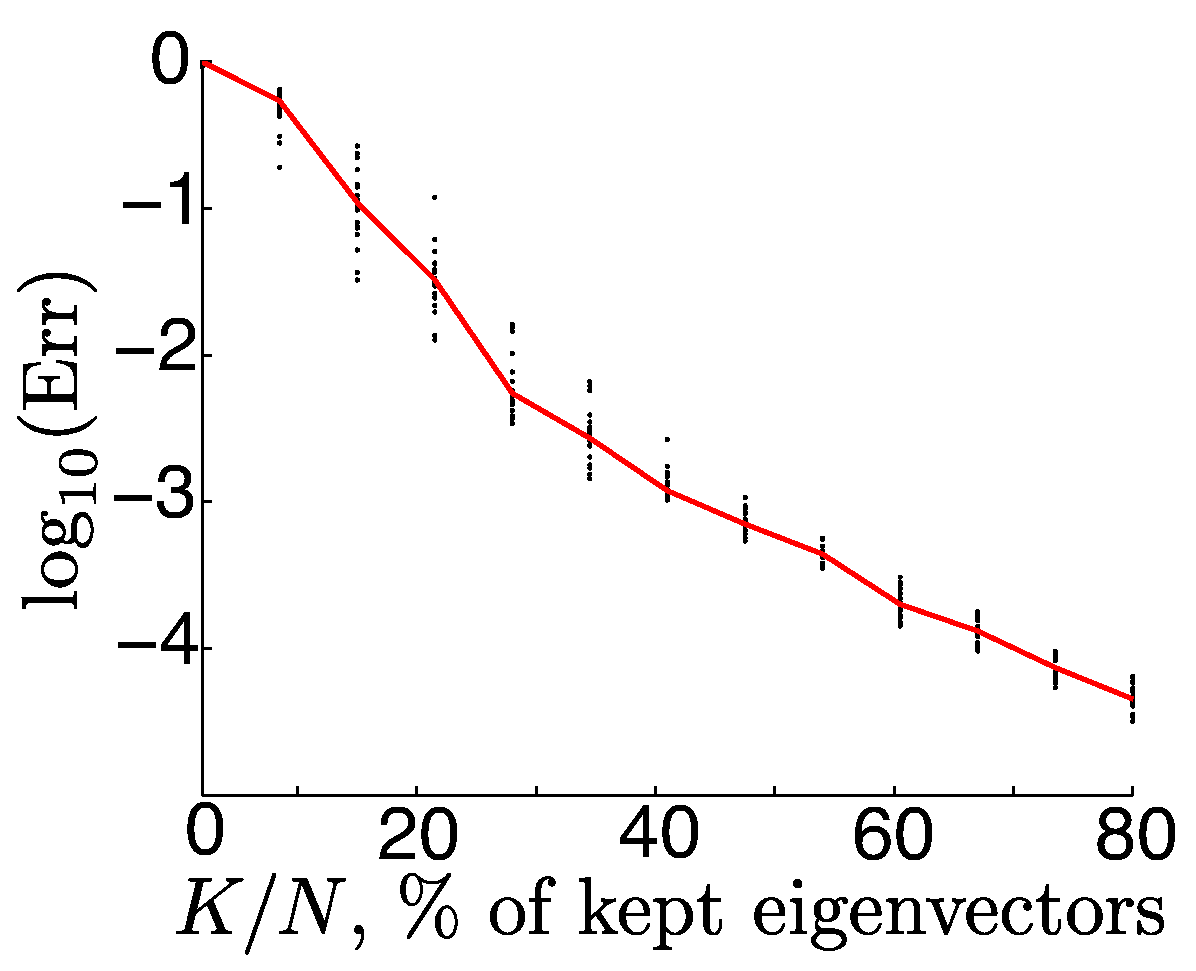
\includegraphics[width=.33\linewidth]{steps-varying-error/steps-varying-cpxity10-error-log.eps}&\hspace{-6mm}
		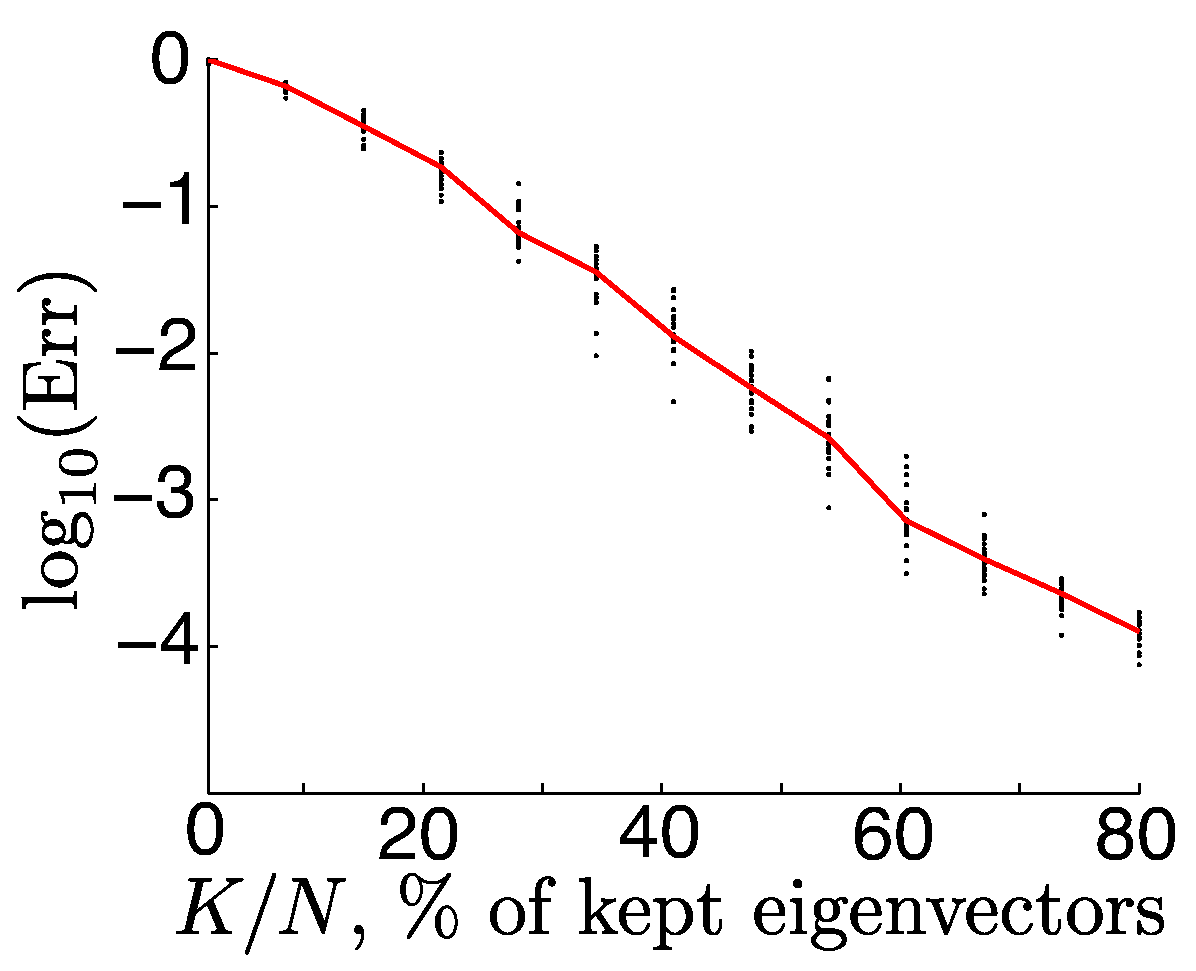
\includegraphics[width=.33\linewidth]{steps-varying-error/steps-varying-cpxity20-error-log.eps}&\hspace{-6mm}
		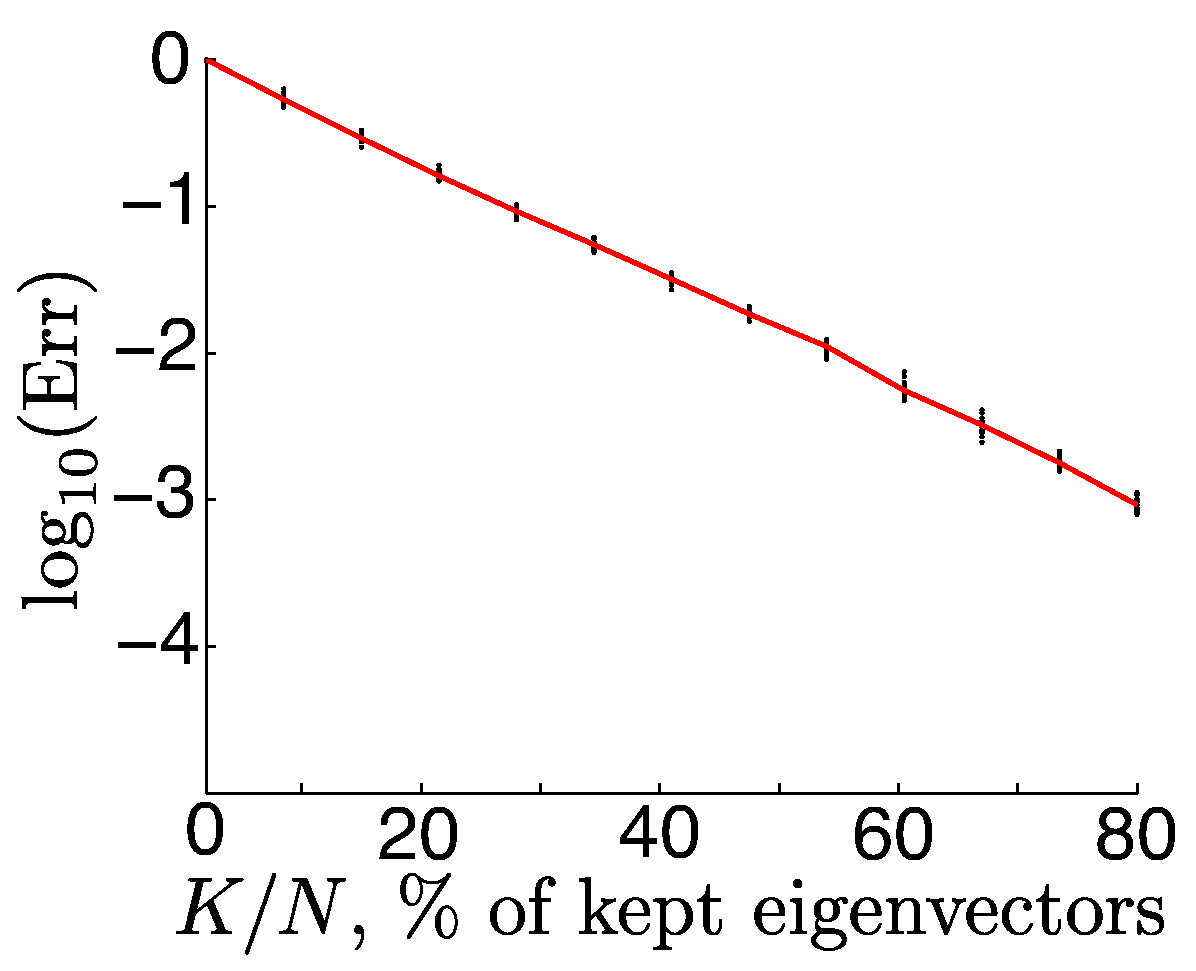
\includegraphics[width=.33\linewidth]{steps-varying-error/steps-varying-cpxity40-error-log.eps}\\
		$\ga=2$ & $\ga=4$ & $\ga=8$	
	\end{tabular}
	\begin{tabular}{c}
    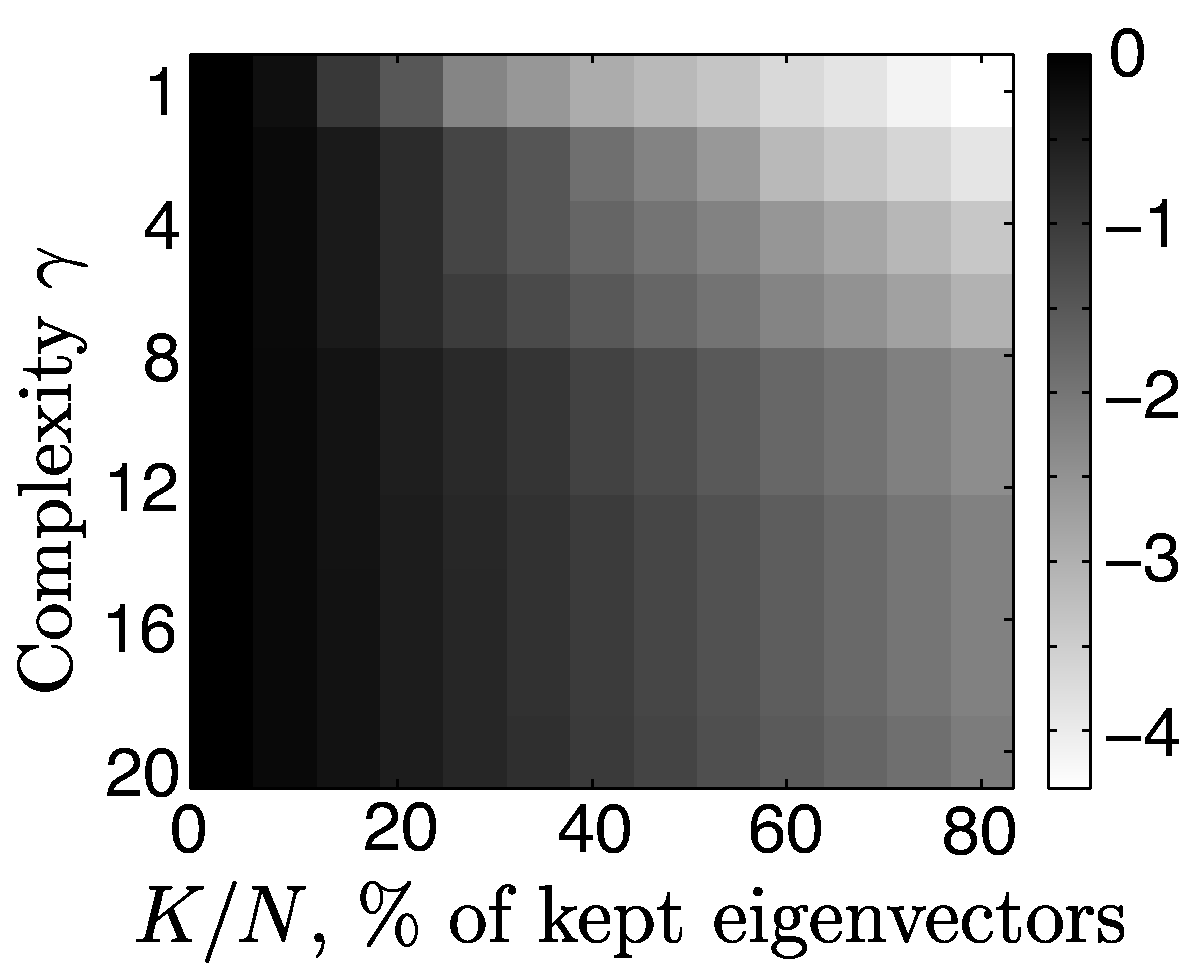
\includegraphics[width=.4\linewidth]{steps-varying-error/steps-varying-all-error.eps}\\
    $\log_{10}(\Err(\si_{\ga},K/N))$
    \end{tabular}
}{ 
	Compressive wave propagation in a piecewise smooth medium. 
}{fig-piecewise-all-error}



%%%%%%%%%%%%%%%%%%%%%%%%%%%%%%%%%%%%%%%%%%%%%%%%%%%%%%%%%
%%%%%%%%%%%%%%%%%%%%%%%%%%%%%%%%%%%%%%%%%%%%%%%%%%%%%%%%%
\subsection{Compressive Reverse-Time Migration}\label{sec:crtm}

In this example, we consider an idealized version of the inverse problem of reflection seismology, where wavefield measurements at receivers are used to recover some features of the unknown impedance $\sigma(x)$. Our aim is to show that compressive wave computation offers significant memory savings in the implementation of a specific adjoint-state formulation that we call \emph{snapshot reverse-time migration}.

%%%%%%%%%%%%%%%%%%%%%%%%%%%%%%%%%%%%%%%%%%%%%%%%%%%%%%%%%
\paragraph{Review of 1D reverse-time migration.}

We will assume a one-dimensional setup as in the rest of this paper, i.e.,
\begin{equation}\label{eq:wave-original}
\sigma^2(x) \frac{\pd^2 u}{\pd t^2} - \frac{\pd u}{\pd x^2} = 0,
\end{equation}
with a known localized initial condition $u(x,0) = u_0(x)$, $\pd u / \pd t(x,0) = u_1(x)$, and over a domain sufficiently large that the choice of boundary conditions does not matter. The $x$ coordinate plays the role of depth. As in classical treatments of reflection seismology, the squared impedance is perturbed about a smooth, known reference medium $\sigma_0^2$, as
\[
\sigma^2(x) = \sigma_0^2(x) + r(x),
\]
where the high-frequency perturbation $r(x)$ has the interpretation of ``reflectors''. The wave equation is then linearized as
\begin{equation}\label{eq:wave-linearized}
\sigma_0^2(x) \frac{\pd^2 u}{\pd t^2} - \frac{\pd u}{\pd x^2} = - r(x) \frac{\pd^2 u_{\mbox{inc}}}{\pd t^2},
\end{equation}
where the incoming field $u_{\mbox{inc}}$ solves the wave equation in the unperturbed medium $\sigma_0^2$. An important part of the seismic inversion problem---the ``linearized problem"---is to recover $r(x)$ from some partial knowledge of $u(x,t)$, interpreted as solving (\ref{eq:wave-linearized}). We will assume the availability of \emph{snapshot} data, i.e., the value of $u$ and $\pd u / \pd t$ at some fixed time $T$,
\[
(d_1(x), d_2(x)) = (u(x,T), \frac{\pd u}{\pd t}(x,T)),
\]
possibly restricted in space to a region where the waves are reflected, by opposition to transmitted. We then let $F[\sigma^2_0]$ for the forward, or modeling operator, to be inverted:
\begin{equation}\label{eq:forward-op}
\begin{pmatrix} d_1 \\ d_2 \end{pmatrix} = F[\sigma^2_0] r.
\end{equation}

A more realistic seismic setup would be to assume the knowledge of $u(0,t)$ for positive $t$, but the step of going from $(d_1, d_2)$ to $u(0,t)$, or vice-versa, is a depth-to-time conversion that should present little numerical difficulty. While assuming trace data $u(0,t)$ would give rise to an adjoint-state wave equation with a right-hand side, working with snapshot data has the advantage of casting the adjoint-state equation as a final-value problem without right-hand side.

More precisely, a simple argument of integration by parts (reproduced in the Appendix) shows that the operator $F$ in (\ref{eq:forward-op}) is transposed as
\begin{equation}\label{eq:imaging-op}
F^*[\sigma^2_0] \begin{pmatrix} d_1 \\ d_2 \end{pmatrix} = - \int_0^T q(x,t) \frac{\pd^2 u_{\mbox{inc}}}{\pd t^2}(x,t)  dt,
\end{equation}
where $q$ solves the adjoint-state equation
\begin{equation}\label{eq:wave-adjoint}
\sigma_0^2(x) \frac{\pd^2 q}{\pd t^2} - \frac{\pd q}{\pd x^2}   = 0,
\end{equation}
with final condition
\[
q(x,T) = \frac{1}{\sigma^2_0(x)} d_2(x), \qquad \frac{\pd q}{\pd t}(x,T) = \frac{-1}{\sigma^2_0(x)} d_1(x).
\]
(notice the swap of $d_1$ and $d_2$, and the minus sign.)

In nice setups, the action of $F^*[\sigma_0^2]$, or $F^*$ for short, called imaging operator, is kinematically equivalent to that of the inverse $F^{-1}$ in the sense that the singularities of $r$ are in the same location as those of $F^*  \begin{pmatrix} d_1 \\ d_2 \end{pmatrix}$. In other words the normal operator $F^* F$ is pseudodifferential. We also show in the Appendix that $F^*$ is the negative Frechet derivative of a misfit functional for snapshot data, with respect to the medium $\sigma^2$, in the tradition of adjoint-state methods \cite{Ple}. Hence applying the imaging operator is a useful component of solving the full inverse problem.

A standard timestepping method is adequate to compute (\ref{eq:imaging-op}); the adjoint wave equation is first solved until time $t = 0$, then both $u$ and $q$ are evolved together by stepping forward in time and accumulating terms in the quadrature of (\ref{eq:imaging-op}). However, this approach is not without problems:
\begin{itemize}
\item The CFL condition restricting the time step for solving the wave equation is typically smaller  than the time gridding needed for computing an accurate quadrature of (\ref{eq:imaging-op}). The potential of being able to perform larger, upscaled time steps is obvious.

\item The backward-then-forward technique just discussed assumes time-reversibility of the equation in $q$ (or conversely of the equation in $u$), a condition that is not always met in practice, notably when the wave equation comes with either absorbing boundary conditions or an additional viscoelastic term. For non-reversible equations, computation of (\ref{eq:imaging-op}) comes with a big memory overhead due to the fact that one equation is solved from $t = 0$ to $T$, while the other one is solved from $t = T$ to $0$. One naive solution is to store the whole evolution; a more sophisticated approach involves using checkpoints \cite{Symes-checkpoint}, where memory is traded for CPU time, but still does not come close to the ``working storage" in the time-reversible case. In this context, it would be doubly interesting to avoid or minimize the penalty associated with time stepping.
\end{itemize}


%%%%%%%%%%%%%%%%%%%%%%%%%%%%%%%%%%%%%%%%%%%%%%%%%%%%%%%%%
\paragraph{Numerical validation of compressive reverse time migration.}

As a proof of concept, we now show how to perform snapshot reverse-time migration (RTM) without timestepping in the case of the reversible wave equation, on a 1D grid of $N=2048$ points. The approach here is simply to compute independently each term of a quadrature of (\ref{eq:imaging-op}) using the compressive wave algorithm for $u$ and $q$. We leave to a future project the question of dealing with 2D and 3D non-reversible examples, but we are confident that most of the ideas will carry through.

The smooth medium $\si_0^2$ is defined as in \eqref{eq-smooth-medium} with $\ga = 1$ (one oscillation) and a contrast $\si_{\max}^2/\si_{\min}^2 = 1.4$. The reflectors $r(x)$ is a sum of two Gaussian bumps of standard deviation $7/N$ and amplitude respectively $-0.6$ and $0.6$, see figure \ref{fig-rtm-error}, top row.

We first compute the input $d_1$ and $d_2$ of the RTM by computing the solution $u(x,t)$ of the wave equation in the perturbed medium $\si^2 = \si_0^2 + r$, and then evaluate $d_1(x) = u(x,T)$ and $d_2(x) = \frac{\partial u}{\partial t} (x,T)$. The initial condition $u(x,0)$ is a second derivative of a Gaussian of standard deviation $7/N$. This simulates seismic observations at time $t=T$, see figure \ref{fig-rtm-error}, top row.  

The algorithm proceeds by computing approximations $\tilde q(x,t_i)$ and $\tilde u_{\text{inc}}(x,t_i)$ of the forward and backward propagations $q$ and $u_{\text{inc}}$ at $N_t=N/10$ equispaced times $\{ t_i \}_{i=0}^{N_t-1}$. These approximations are computed for each $t_i$ independently, without time stepping, by using the compressive algorithm with a small set of $K < N$ eigenvectors. The RTM estimation of the residual $r(x)$ is obtained by discretizing \eqref{eq:imaging-op}
\eq{
	\tilde r(x) = 
	- \frac{1}{n_t} \sum_{i=0}^{n_t-1} \tilde q(x,t_i) \frac{\pd^2 \tilde  u_{\mbox{inc}}}{\pd t^2}(x,t_i),
}
where the derivative is computed using finite differences. 

The success of compressive RTM computations is measured using an error measure $\Err(K/N)$ obtained similarly to \eqref{eq-error-measure} by averaging over several randomizations for the sets $\Om \in \Om_K$ of $|\Om|=K$ eigenvectors
\eq{
	\Err(K/N)^2 = \frac{1}{N |\Om_K| \, \norm{u}} \sum_{\Om \in \Om_K} \sum_{j=0}^{N-1} | \tilde r_0[j] - \tilde r[j] |^2 
}
where $\tilde r_0$ is the RTM estimation obtained with the full set of $N$ eigenvectors.

Figure \ref{fig-rtm-error}, bottom row, displays the decay of $\Err(K/N)$ with the number of eigenvectors used for the compressive computations. This shows that roughly $20\%$ of eigenvectors are needed to reach 1 digit of accuracy, and $30\%$ to reach 2 digits of accuracy.

Note that this simple RTM method cannot be expected to recover the original $r(x)$ accurately, mainly because we have not undone the action of the normal operator $F^* F$ in the least-square treatment of the linearized problem.

Also note that the compressive algorithm was run ``as is", without any decomposition of the initial condition, or split of the time interval over which each simulation is run, as in Section \ref{sec:sparsity-enhancement}.

\myfigure{
	\begin{tabular}{cc}
    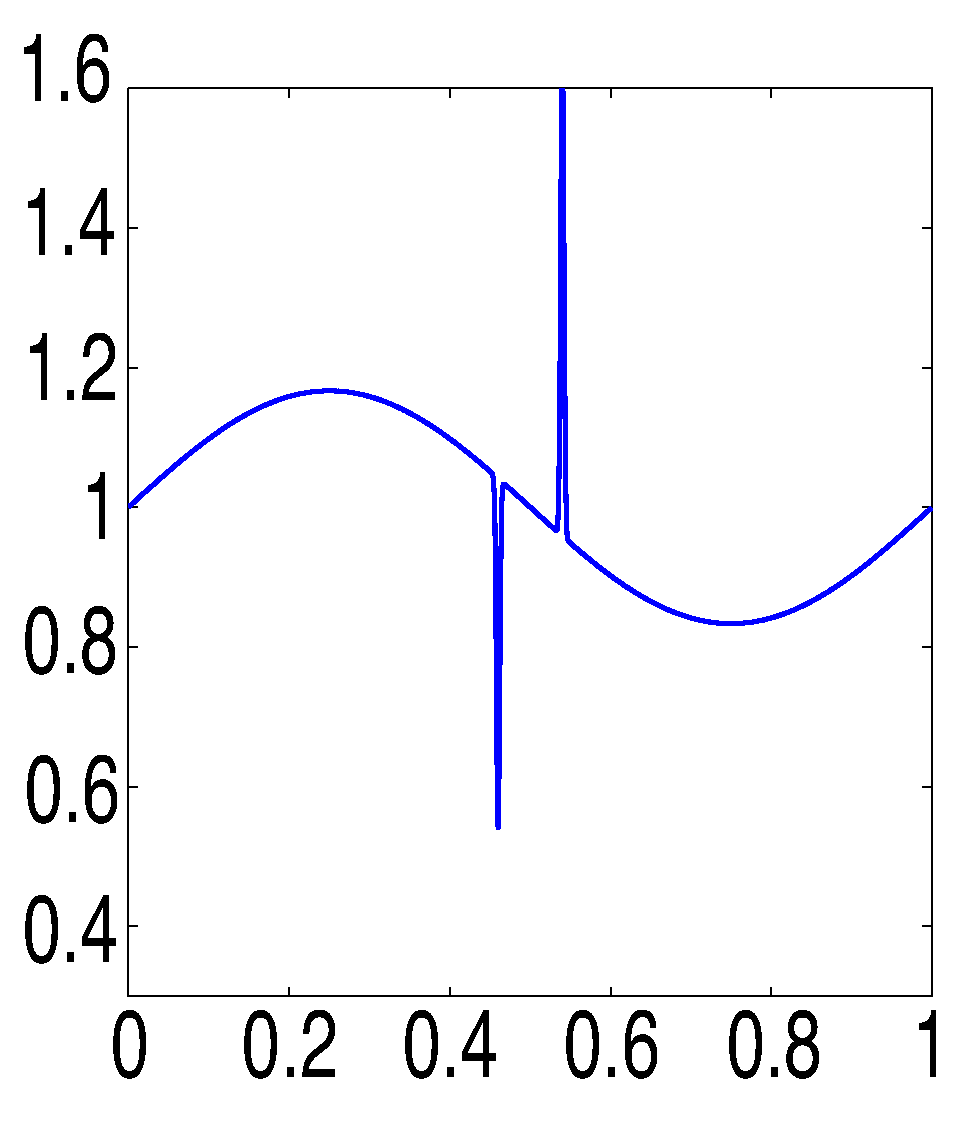
\includegraphics[width=.35\linewidth,height=.25\linewidth]{rtm/twodiracs-rtm-speed-c.eps}&
    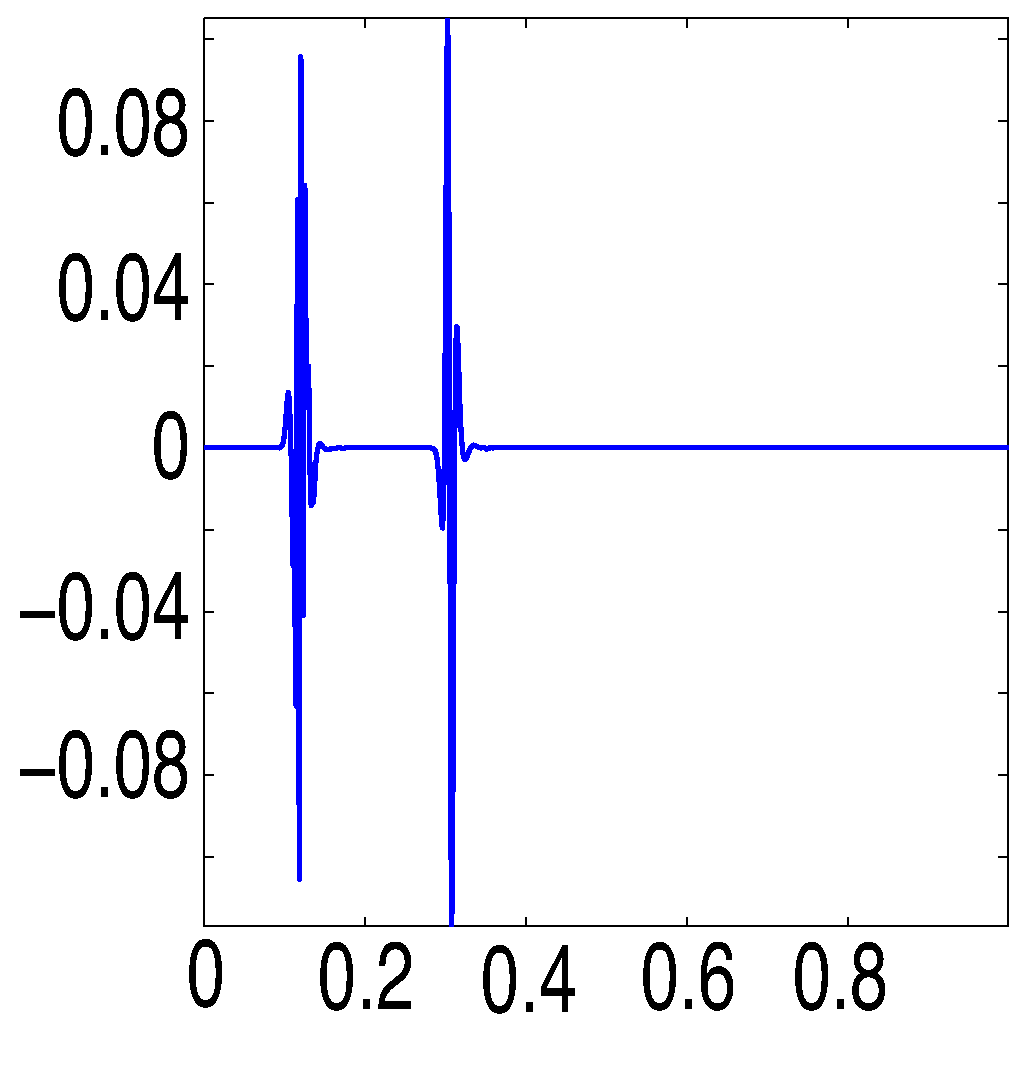
\includegraphics[width=.35\linewidth,height=.25\linewidth]{rtm/twodiracs-rtm-reflec-wave.eps}\\
    $\si^2 = \si_0^2 + r$ & $d_1$
    \end{tabular}
    \\
	\begin{tabular}{cc}
    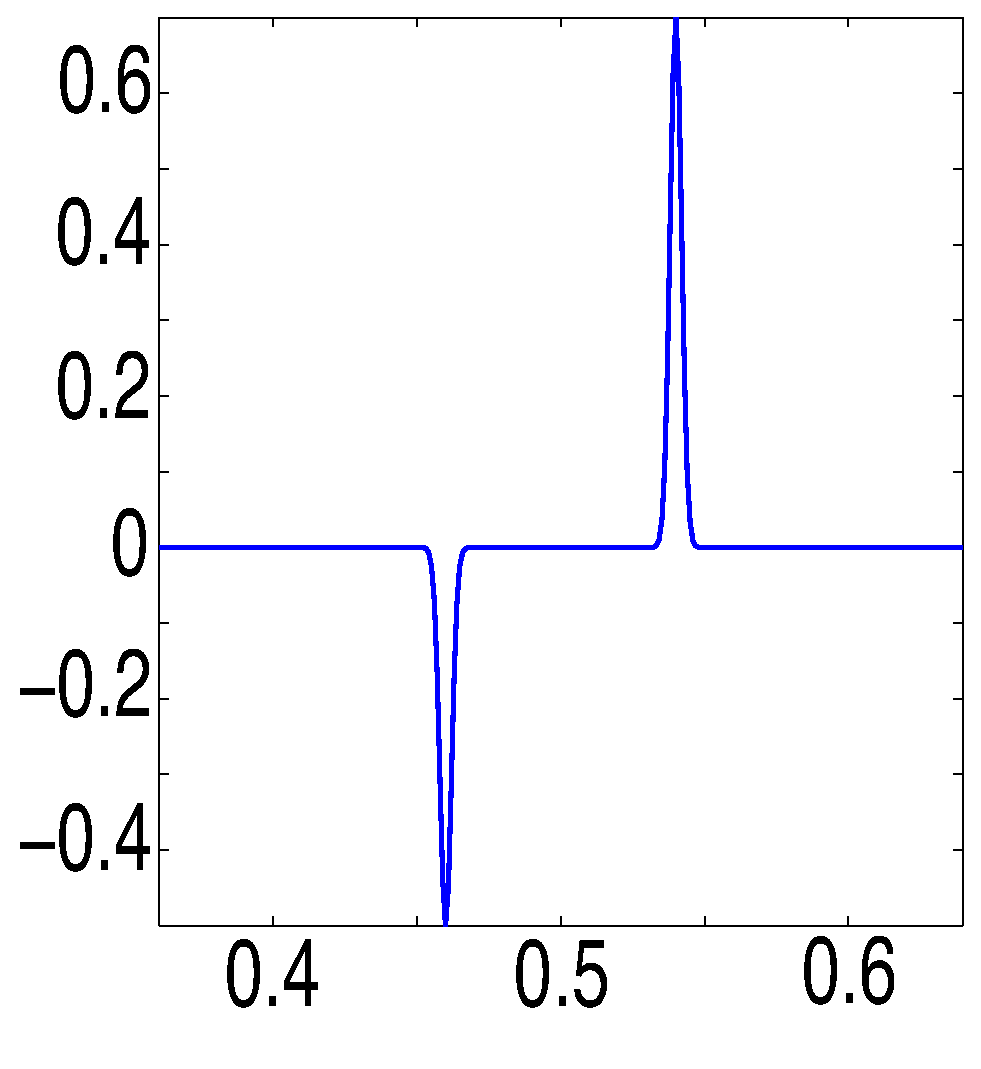
\includegraphics[width=.35\linewidth,height=.25\linewidth]{rtm/twodiracs-rtm-residual-zoom.eps}&
    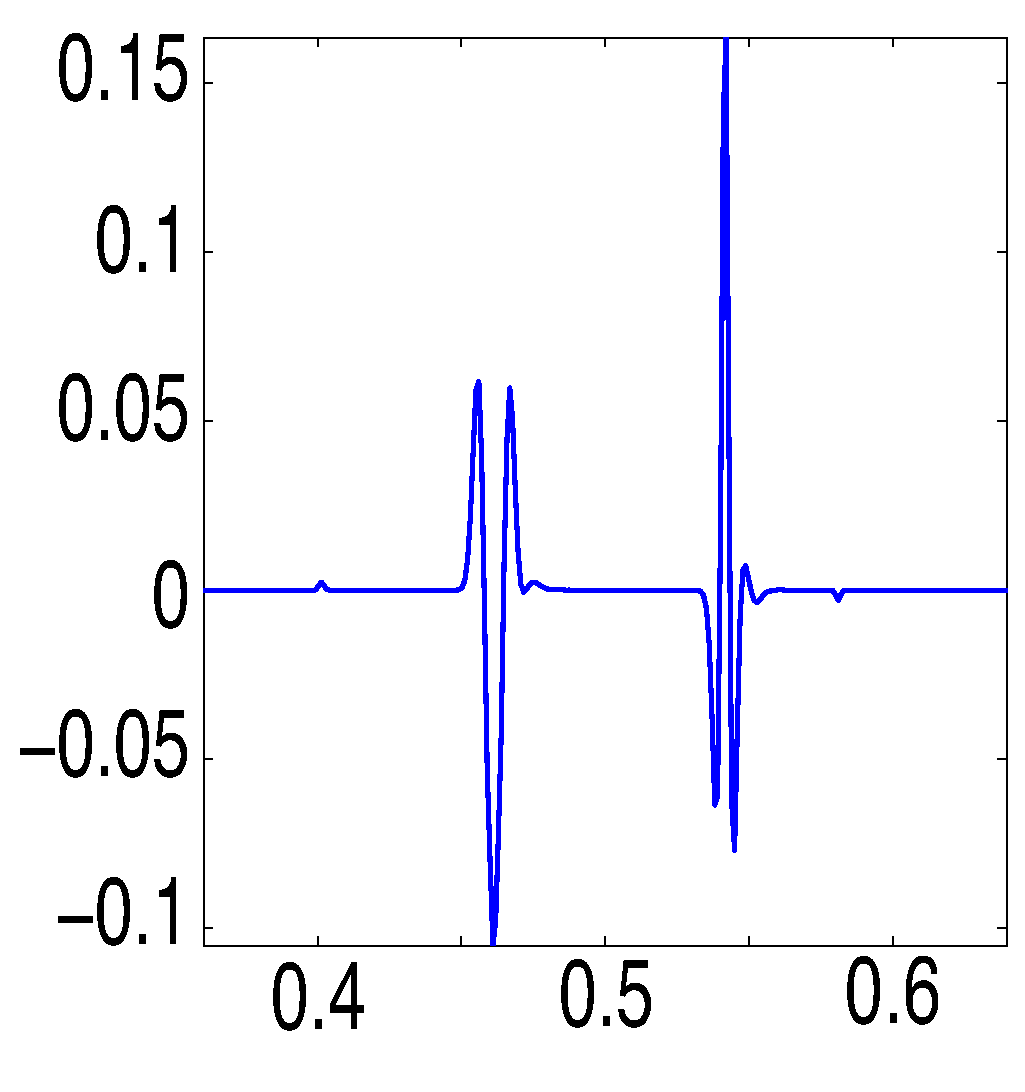
\includegraphics[width=.35\linewidth,height=.25\linewidth]{rtm/twodiracs-rtm-zoom.eps}\\
    $r(x)$ (zoom) & $\tilde r(x)$ (zoom)
    \end{tabular}
    \\
	\begin{tabular}{c}
    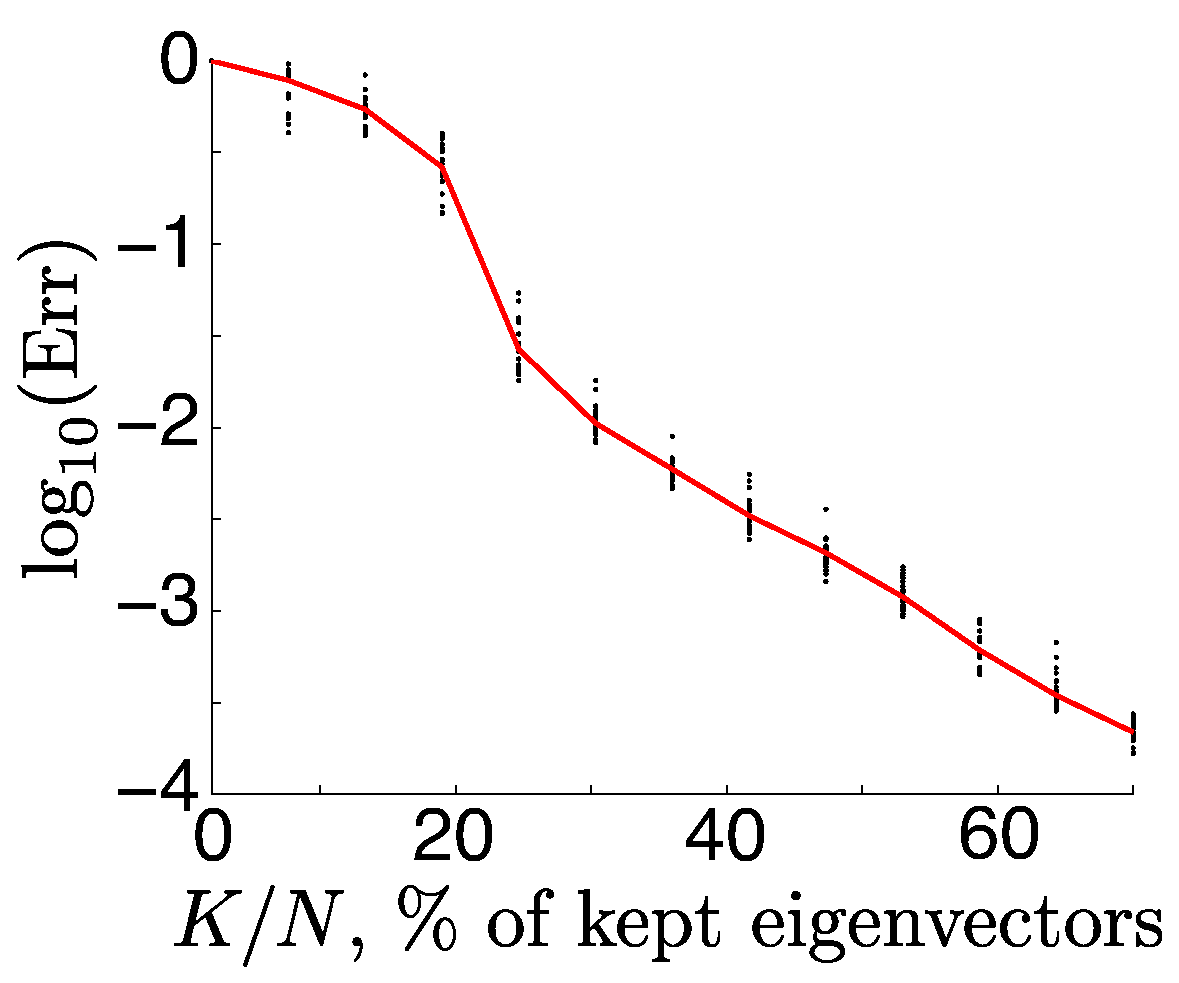
\includegraphics[width=.4\linewidth]{rtm/twodiracs-rtm-error-log.eps}\\
    $\log_{10}(\Err(K/N))$
    \end{tabular}
}{ 
	Top row: perturbed speed $\si^2$ and input $d_1$ of the RTM computations.
	Middle row: reference solution $r_{\text{RTM}}$ and approximated solution $\tilde r_{\text{RTM}}$ for $K/N = 0.2$.
	Bottom row: recovery error decay $\log_{10}(\Err(K/N))$ as a function of the sub-sampling $K/N$. Each black dot corresponds to the error of a given random set $\Om$ (the red curve is the result of the averaging among these sets).
}{fig-rtm-error}


